% Dokumenteinstellungen
% ======================================================================

% Die Dokumentklasse definiert die Art des Dokuments
% und seine Grundeigenschaften
\documentclass[11pt,a4paper]{scrartcl}		% [Schriftgröße 10, Textbereich Din A4] {Dokumentart Artikel}


% Zusätzliche (aber sinnvolle) Pakete laden
% ======================================================================
% Pekete fügen verschiedene Funktionen zu LaTeX hinzu.
% ganz ohne Pakete wäre Latex gerade mal etwas besser als notepad...
\usepackage[a4paper]{geometry}				% DIN-A4 Größe des Papiers; sollte mit der Ausdehnung des Textes in documetnclass übereinstimmen.
\usepackage[utf8]{inputenc}					% Zeichenkodierung UTF-8 falls Probleme wegen utf8 auftreten, utf8 durch utf8x ersetzen
\usepackage[T1]{fontenc}
\usepackage{lmodern}
\usepackage{amsmath}						% erlaubt mathematische Formeln
\usepackage[english]{babel}					% Deutsche Sprache und Silbentrennung
\usepackage{amssymb}						% Verschiedene Symbole
\usepackage{graphicx}						% Zum Bilder einfügen benötigt
\usepackage{hyperref}						% Sprunglinks für Überschriften, Fußnoten und Weblinks

%Eigenes

\usepackage{subfig}							% Subfloat Benutzung, Unterteilung für Bilder

\usepackage[numbers,square]{natbib}
\bibliographystyle{alphadin}%plaindin}%unsrt}%alphadin}
\usepackage{gensymb}
\usepackage{setspace}
\usepackage{geometry}
\geometry{a4paper,left=2.5cm,right=2.5cm}

\usepackage{siunitx}
\usepackage{booktabs}
\usepackage{eurosym}

\usepackage[shortlabels]{enumitem}

\usepackage{fixltx2e}  % Für \textsubscript{}

\usepackage{tabularx}
\newcolumntype{L}[1]{>{\raggedright\arraybackslash}p{#1}}
\newcolumntype{R}[1]{>{\raggedleft\arraybackslash}p{#1}}
\newcolumntype{C}[1]{>{\centering\arraybackslash}p{#1}}

\usepackage{longtable}

\usepackage{pdfpages}

\usepackage{pstricks}	% Erstellung von Plots
\usepackage{pst-plot}



% Dokumentbeginn
% ======================================================================
% Ab hier beginnt das eigentliche Dokument.
% Alles was danach folgt wird im fertigen PDF angezeigt.

\begin{document}


% Titelblatt
% ===========================================

\begin{titlepage}
	
	\singlespacing
	\begin{center}
	
		\quad
		\vspace{1cm}
	
		\Large{\textbf{Project Work\\Cyber-Physical Systems}}
	
		\vspace{1.5cm}
	
		\huge{\textbf{Autonomous Aerobatics on\\Commanded Paths}}
	
		\vspace{1.5cm}
	
		written by
		
		\vspace{1.5cm}
	
		\Large{\textbf{Youlin Gao\\Anthony Blanc\\Andreas Bruckmeier}}
	
		\vfill
		
		submitted at the\\
		Institute for Real-Time Computer Systems\\
		Technische Universität München,\\
		to\\
		Prof. Marco Caccamo

		\vspace{1cm}		
		
		Date: 26th February 2016
	
	\end{center}
	
\end{titlepage}

\setstretch{1.2}


% Inhaltsverzeichnis   (Überschriften werden automatisch in das Inhaltsverzeichnis aufgenommen.)
% ===========================================
\newpage
\tableofcontents	

\vfill

% Abbildungsverzeichnis
% ===========================================

%\renewcommand{\listfigurename}{}
\listoffigures
%{\def\section*#1{}\listoffigures}


% Textbeginn
% ================================================================================
% ================================================================================


% Neue Seite
% ===========================================
\newpage
	

\section{Overview}

As a part of the CPS course in WS15/16, a controller structure for an aircraft in an simulation environment was built, performing autonomous aerobatics on commanded paths.
In this report, the controller structure is explained and achievements are presented.
Before, an overview of the features are given and the underlying work is clarified.

\medskip






\subsection{Working Principle and Features}

Control target of the controller is a path in 3-dimensional space as a function of time.
The controller's aim is to fly along this commanded path by determining the deviation from the given trajectory and thereout calculating acceleration commands which are the inputs of the actuator-controllers of the aircraft.

\textbf{Figure~\ref{fig_complete_structure}} depicts the complete control structure of the aerobatic controller. 
With the position data of the trajectory and actual position signals of the aircraft, the desired acceleration is computed, and by considering the gravity handed to the control structure where the acceleration in body frame is used as the control variable for the aileron-, elevator-, and rudder-control.
Also, with the position data, the delay of the aircraft from the desired path is determined and by considering a look ahead distance, the throttle is controlled with this information.

The resulting steering signals computed by the control structure are handed to the simulation environment which hands back measurement results of the virtual aircraft's sensors.
These signals are processed and provided to the control structure. A feature of the signal processing is the estimation of the aircraft-position with accelerometers and gyrometers when there is no available GPS-signal.

\begin{figure}[!h]
  \begin{center}
  	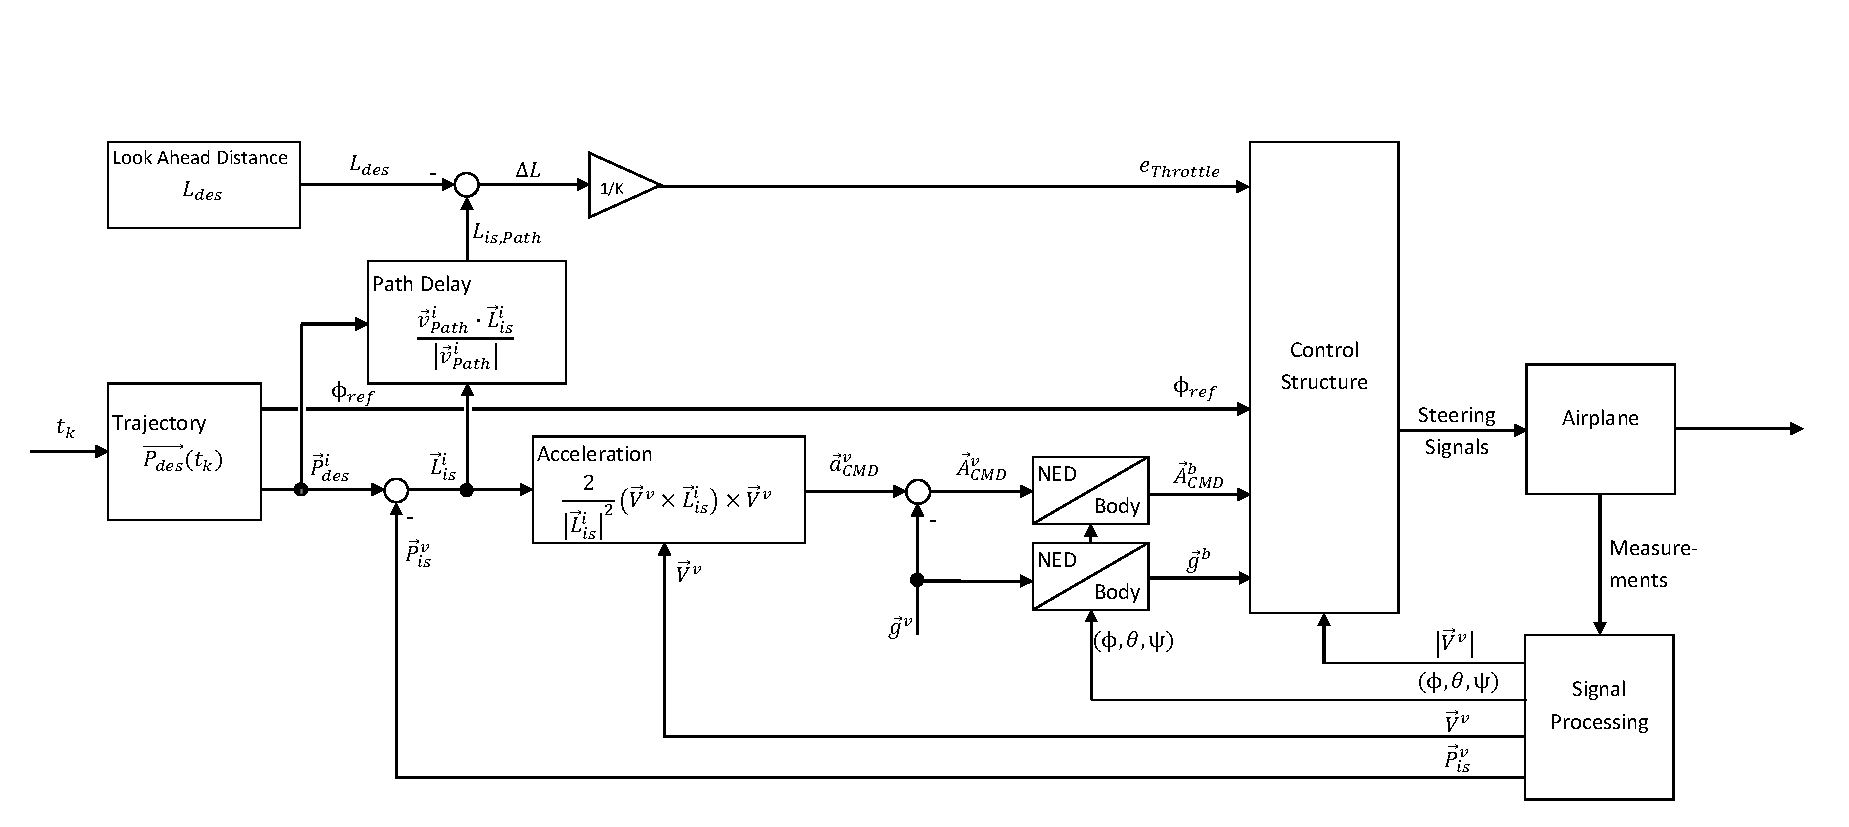
\includegraphics[width=18cm, angle=90]{pictures/complete_structure.pdf}
  \end{center}
  \caption{Overview of the control structure of the aerobatic controller.}
  \label{fig_complete_structure}
\end{figure}


\subsection{Underlying Work}

The control structure, implemented and presented in this project work, is based on the work of Sanghyuk Park\cite{Park.2012} and modified by establishing the desired path depending on time and determining the path delay in order to control the throttle.

The estimation of the aircraft's position signal is implemented after a method which is, at the time of handing in this report, not yet published. We got the access ahead to the release by our tutor.

\medskip





\section{Details}

In the following, each part of the control structure (compare Figure~\ref{fig_complete_structure}) is presented in detail.

\medskip





\subsection{Interface with the Simulation Environment}

The interface of our program with the simulation environment is at the beginning of each program run, when sensor data is handed over.
The function~\textsf{calculateStateVariables} reads this sensor data  to our program.

At the end of each program run, the four steering signals for the actuators throttle, aileron, rudder, and elevator are given to the simulation environment in the function~\textsf{generateOutSignals} and the following instructions \textsf{hal.rcout}.

\medskip




\subsection{User Interface}

We have implemented an user interface which enables a communication with the aircraft controller via the USB connection with the controller board. 
We used the program \texttt{hterm} for communicating with the controller over a COM-Port.

The interface enables the user to modify controller parameters and flight paths at run time by sending following instructions:
\begin{itemize}
\item 
instruction 1
\item
instruction 2
\end{itemize}

\medskip




\subsection{Path Generation}



\medskip





\subsection{Processing of Control Variables}

\subsubsection*{Processing the Sensor Data}

\subsubsection*{Computing the Desired Acceleration}

Introduce look ahead distance, explain, why important -> $L_is$ is always > 0 and ensures a good acceleration command

\subsubsection*{Determining the Desired Speed}\label{ch-Determ-Desired-Speed}

The desired speed of the aircraft is given implicitly with the desired path and can be gathered by calculating the derivative of $\vec{P}_{des}^i$:
\begin{equation}
\vec{v}_{Path}^i(t_k) = \frac{\vec{P}_{des}^i(t_k)-\vec{P}_{des}^i(t_{k-1})}{\Delta T}\quad .
\end{equation}

But the desired speed is not the control variable of the throttle controller. As shown in Figure~\ref{fig_complete_structure}, the input for the throttle controller is $\Delta L$ which is the distance of the aircraft from the desired position with respect to the look-ahead distance~$L_{des}$ and is computed by
\begin{equation}
\Delta L = \frac{\vec{v}_{Path}^i \cdot \vec{L}_{is}^i}{|\vec{v}_{Path}^i|}-L_{des} = L_{is,Path}-L_{des} \quad .
\end{equation}
Here, $L_{is,Path}$ is the distance of the aircraft concerning/on the desired flight direction expressed in $\vec{v}_{Path}^i$.
This relation is shown graphically in \textbf{Figure~\ref{fig_explanation-diagram-throttle}}. The inner structure of the component \texttt{Path Delay} is depicted in \textbf{Figure~\ref{fig_Path_Delay}}.
Finally, $\Delta L$ is divided by a constant value~$K$ and handed to the throttle controller as input $e_{Throttle}$ (see Figure~\ref{fig_Control-Structure}).

\begin{figure}[tbh]
  \begin{center}
  	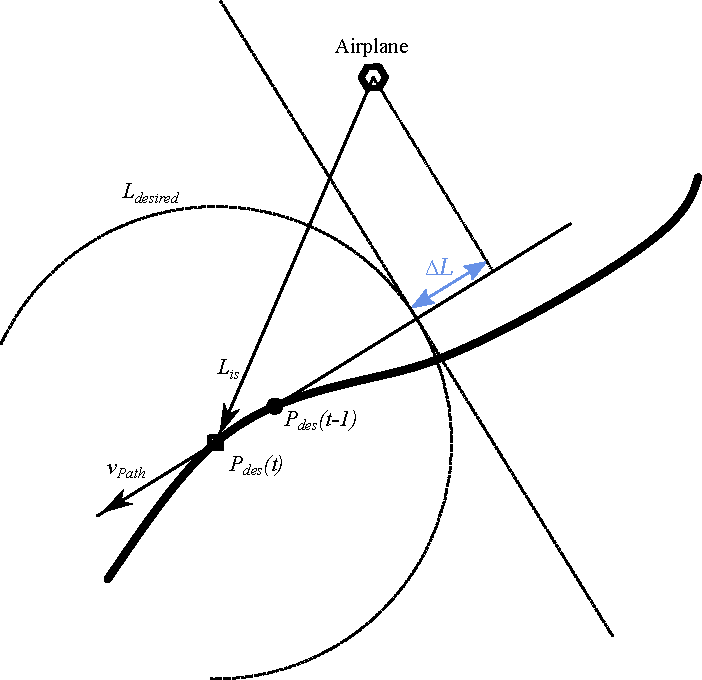
\includegraphics[width=8cm]{pictures/explanation-diagram-throttle.pdf}
  \end{center}
  \caption{Determination of the input for the throttle-controller $\Delta L$.}
  \label{fig_explanation-diagram-throttle}
\end{figure}

\begin{figure}[tbh]
  \begin{center}
  	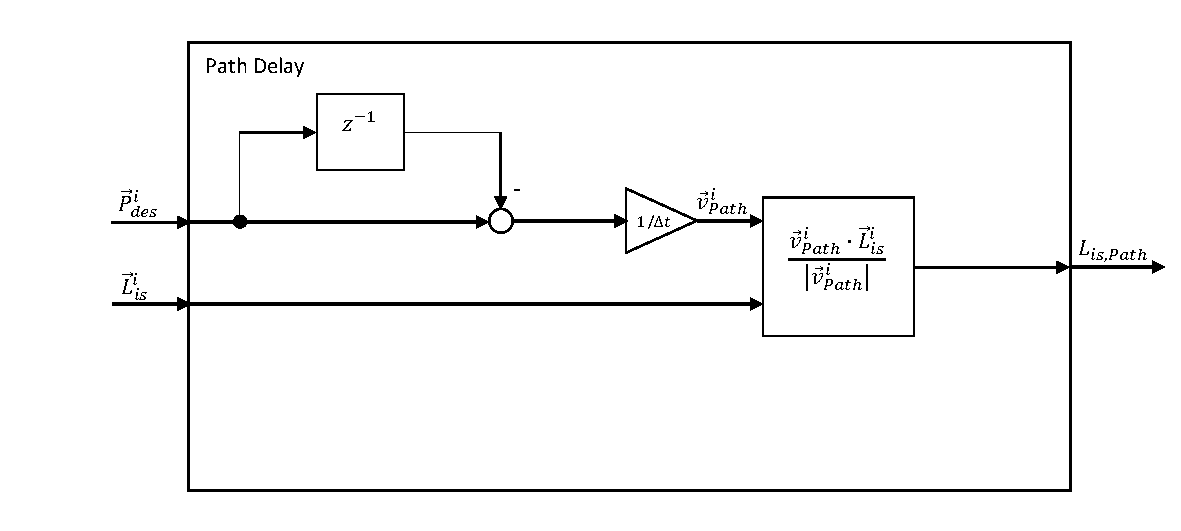
\includegraphics[width=12cm]{pictures/Path_Delay.pdf}
  \end{center}
  \caption{Inner structure of the component \texttt{Path Delay}.}
  \label{fig_Path_Delay}
\end{figure} 

With this control mechanism, the aircraft will adjust the throttle in order to always stay behind the desired position by the length of the look ahead distance~$L_{des}$ which is the intersection of the desired flight direction~$\vec{v}_{Path}^i$ and the circle of $L_{des}$ as shown in Figure~\ref{fig_explanation-diagram-throttle}. In this point, $\Delta L$ will become zero, which is the control target of the control structure (of course, the whole tangent of the intersection point will meet the control target of $\Delta L = 0$ but the rest of the control structure will force the aircraft onto the desired path and thus to this one intersection point).  

\medskip





\subsection{Control Structure}

In the \texttt{Control Structure}, the four actuators of the aircraft, namely throttle, aileron, rudder, and elevator, are regulated by PID-controllers with a error~$e$ value as input:
\begin{equation}
output(t) = K_p \cdot E(t) + K_i \cdot \int_{t_0}^t E(\tau)\, \mathrm{d}\tau + K_d \cdot \frac{\mathrm{d}}{\mathrm{d}t}E(t)\quad .
\end{equation}

\subsubsection*{Throttle}
The input error of the throttle is the sum of current aircraft velocity~$|\vec{V}^v|$ and the distance of the aircraft~$e_{Throttle}$, lagging behind the desired point, as described in Section~\ref{ch-Determ-Desired-Speed}. 
\begin{equation}
E_{throttle} = |\vec{V}^v| + e_{Throttle}
\end{equation} 
The addition of the aircraft velocity is for keeping the engine speed at the desired level, only the error term can increase or decrease the engine speed.

\subsubsection*{Aileron}
The aileron controller is implemented as described in the work of S.~Park\cite[p.~71]{Park.2012}.
A reference vector~$\hat{e}_{roll}$, always pointing out of the roof of the aircraft, is compared with the acceleration command~$\vec{A}_{CMD}^b$. 
The control target is to let both vectors point into the same direction (this is shown graphically in the paper of S.~Park on page~70~\cite{Park.2012}.
Mathematically, this is achieved with following equation:
\begin{equation}
E_{aileron}=\arcsin\left(\hat{e}_{roll} \times \frac{\vec{A}_{CMD}^b}{|\vec{A}_{CMD}^b|}\right)_x
\end{equation}
The reference vector~$\hat{e}_{roll}$ can be modified by the angle~$\phi_{ref}$. At the value of $\phi_{ref}=90\degree$, $\hat{e}_{roll}$ is pointing out of the right wing of the aircraft; at $\phi_{ref}=180\degree$, the reference vector is pointing out of the fuselage.
This can be used for performing a roll manoeuvre.

\subsubsection*{Rudder and Elevator}
Rudder and elevator are controlled with the acceleration command~$\vec{a}_{CMD}^b$, which does not contain the gravity term~$\vec{g}^b$.
The rudder control takes the y-component as input, and the elevator control uses the z-component:
\begin{equation}
E_{rudder}=(\vec{a}_{CMD}^b)_y\quad , \quad E_{elevator} = (\vec{a}_{CMD}^b)_z
\end{equation}

The \texttt{Control Structure} is depicted in symbolic form in \textbf{Figure~\ref{fig_Control-Structure}}.

\begin{figure}[tbh]
  \begin{center}
  	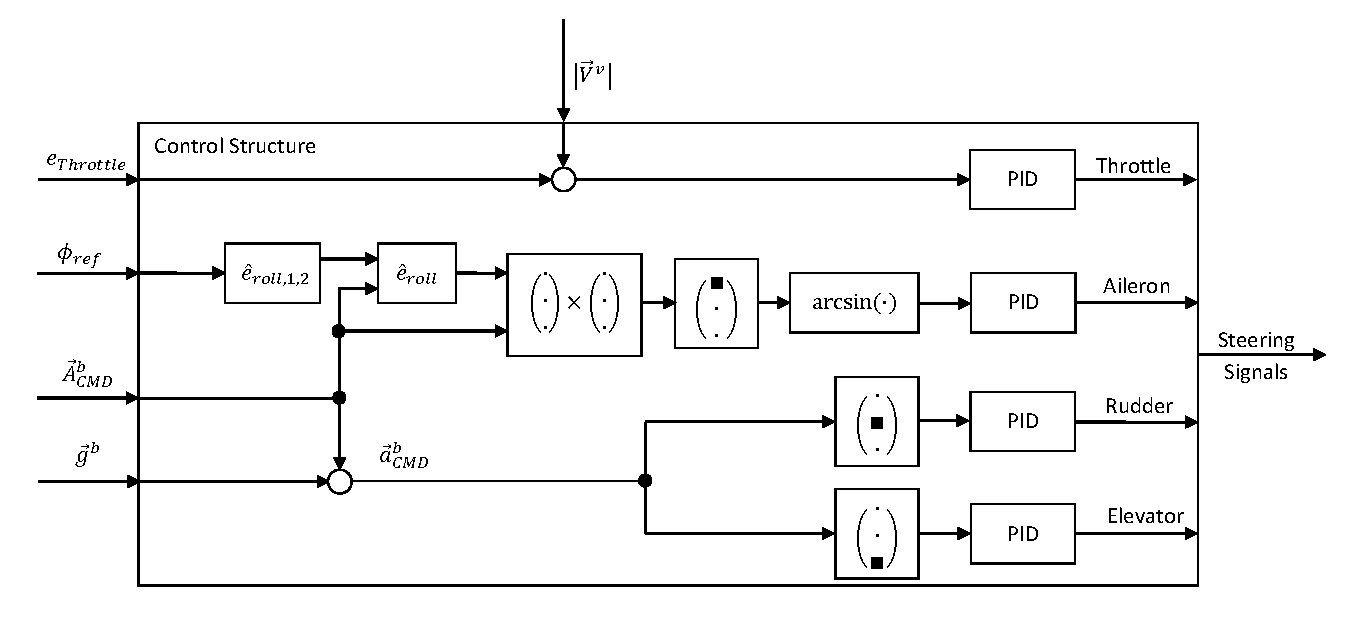
\includegraphics[width=12cm]{pictures/PID.pdf}
  \end{center}
  \caption{Inner structure of the component \texttt{Control Structure}.}
  \label{fig_Control-Structure}
\end{figure}


\medskip






\subsection{GPS Signal Estimation}

In the case of an inverted flight attitude, a GPS-signal cannot be received due to GPS-receivers not pointing to the sky.
Therefore, the position of the aircraft has to be estimated with data of measuring instruments, still available, which is data from the accelerometer and the gyrometer.
However, in the simulation, position data is always provided, so an inverted flight attitude has to be detected and position signals have to be ignored in order to realise a real GPS-signal.

\smallskip

Therefore, a function is implemented, which observes the euler angles of the aircraft, which indicate the flight attitude of the aircraft.
As soon as the roll angle or heading angle has an amount greater than $60\degree$, the function activates the position estimation and overwrites the position signals.

\smallskip

The position estimation principle is an integration method.
First, the derivatives of the Euler angles are computed with the available rotation rates. 
Those derivatives are time-step integrated to obtain the Euler angles, e.g.:
\begin{equation}
 \phi_{t_k} = \frac{1}{2}(\dot{\phi}_{t_k}+\dot{\phi}_{t_{k-1}})\cdot \Delta T + \phi_{t_k}
\end{equation}

In the next step, the acceleration of the aircraft is depicted with the data of the accelerometer plus data of the rotation rates.
With the same time-step integration method as shown above, the aircraft-velocity, and with a further integration step, the position is obtained.

\smallskip

As soon as the aircraft is able to receive a GPS-signal, the estimation is switched off and the measured position data is taken, again.


\medskip





\section{Results}


In summary, the presented and implemented control structure showed very good results for various aerobatic manoeuvres which are shown in the following.

\medskip

But beforehand, it is to mention that the rudder was not activated as the results were recorded.
The reason was a faulty adapter software which caused a disconnection with the controller after a few seconds of flight. Instead, we used a stable working adapter software which did not support the control of the rudder.

Also, the GPS signal estimation could not be activated due to imprecise estimation results.
The reasons were the lack of information about the used units of the measurement data and the position of the accelerometers in the aircraft which has to be considered in a compensation term.

\bigskip






% Textende
%----------------------------------------------------------------
%----------------------------------------------------------------
% Anhang

\newpage

\begin{appendix}
%\renewcommand{\refname}{A}
\section{Appendix}

\bigskip



% Literatur
% ===========================================
\subsection{References}

\begin{flushleft}
\renewcommand{\refname}{}
\singlespacing
%\bibliography{references}
{\def\section*#1{}\bibliography{references}}
\end{flushleft}

%\newpage


\bigskip

\subsection{Notation}

\begin{tabbing}
	 \hspace{2cm} \= \hspace{2cm} \= \hspace{3cm} \kill
	\> $t_k$ \> Point in time (time-discrete)\\	
	\> $\Delta T$ \> Time period of one time step of the system\\
	\> $\phi_{ref}$ \> Angle of reference vector for aileron control, forces the roll-angle\\
	\> $\vec{P}_{des}^i$ \> Desired position of the aircraft (inertial frame)\\
	\> $\vec{P}_{is}^i$ \> Actual position of the aircraft (inertial frame)\\
	\> $\vec{L}_{is}^i$ \> Difference between desired and actual position (inertial frame)\\
	\> $\vec{a}_{CMD}^v$ \> Desired Acceleration of the aircraft (vehicle frame)\\
	\> $\vec{g}^{v,b}$ \> Acceleration by gravity (vehicle,body frame)\\
	\> $\vec{A}_{CMD}^{v,b}$ \> Desired Acceleration with gravity considered (vehicle,body frame)\\
	\> $L_{des}$ \> Look-ahead distance \\
	\> $L_{is,Path}$ \> Distance concerning the desired path, the aircraft lags behind \\
	\> $\Delta L$ \> Desired distance the aircraft needs to catch up \\
	\> $e_{Throttle}$ \> Input error for the throttle controller \\
	\> $(\phi,\theta,\psi)$ \> Euler angles of the aircraft \\
	\> $\vec{V}^v$ \> Velocity vector of the aircraft (vehicle frame)\\	
	
\end{tabbing}


\end{appendix}

\end{document}


% -------------------Bausteine--------------------------------------
	
%\begin{figure}[!b]
%  \begin{center}
%    \includegraphics[width=16cm]{../Machine-Epsilon-different-divisors.eps}
%  \end{center}
%  \caption{\small Figure caption. To get a figure to span two
%      columns, use the environment figure* rather than figure.}
%  \label{fig-label}
%\end{figure}


%\begin{enumerate}[{(\arabic{enumi})}]
%
%	\item
%			
%\end{enumerate}

%\begin{pspicture}[xAxisLabel=Auslastung,yAxisLabel=Herst.-Kosten](-0.5,0)(0.5,6.5)
%\begin{psgraph}[arrows=->,Dx=1,Dy=2](0,0)(-0.1,-0.1)(1.2,1.2){5cm}{4cm}
%	\psplot[plotpoints=200,linecolor=red]{0.075}{1}{0.2 0.1 x add div}
%\end{psgraph}
%\end{pspicture}

%\begin{figure}[ph]
%	\centering
%	\caption{Function with three different solvers for task~2.}
%	\lstinputlisting{../Solver.m}
%	\label{Code-Solver}
%\end{figure}

	
%\section{Literature}
%
%\renewcommand{\refname}{}
%
%\begin{flushleft}
%
%\singlespacing
%\bibliography{references}
%
%\end{flushleft}

%\begin{figure}[ph]
%	\centering
%	\subfloat[Forward Euler]{
%		\includegraphics[width=7.5cm]{../02-FE.eps}
%	}
%	\hfill
%	\subfloat[Symplectic Euler]{
%		\includegraphics[width=7.5cm]{../02-SE.eps}
%	}
%	\\
%	\centering
%	\subfloat[Stormer-Verlet]{
%		\includegraphics[width=7.5cm]{../02-SV.eps}
%	}
%	\hfill
%	\subfloat[Monat November]{
%		\includegraphics[width=7.5cm]{../02-err.eps}
%	}
%	\hfill
%	\caption{Solutions of the computed methods in task~2.}
%	\label{02}
%\end{figure}

%\renewcommand{\arraystretch}{1.4}
%\begin{table}[ht]
%\caption{Simulierte Szenarien.}
%\centering
%\begin{tabular}{R{5cm}|cc}
%\toprule 
%\textbf{Größe} & \textbf{Formelzeichen} & \textbf{Einheit} \\
%\midrule
%\textbf{Strahlungsfluss} & $\Phi_e$ & $\SI{}{\watt}$ \\
%\textbf{Bestrahlungsstärke} & $E_e = \frac{\mathrm d \Phi_e}{\mathrm d A}$ & $\SI{}{\watt \per \square \meter}$ \\
%\textbf{Lichtstrom} & $\Phi$ & $\SI{}{\lumen}$ \\
%\textbf{Beleuchtungsstärke} & $L = \frac{\mathrm d \Phi}{\mathrm d A}$ & $\SI{}{\lux} = \SI{}{\lumen \per \square \meter}$ \\
%\textbf{Lichtausbeute} & $K = \frac{\Phi}{P}$ & $\SI{}{\lumen \per \watt}$ \\
%\bottomrule 
%\end{tabular}
%\label{tab:groessen-einheiten}
%\end{table}
%\renewcommand{\arraystretch}{1.0}